\documentclass[12pt, a4paper]{article}
\usepackage[czech]{babel}

\usepackage{graphicx}
\usepackage{subcaption}
\usepackage{parskip}
\usepackage{longtable}
\usepackage{amsmath}
\usepackage{float}
\usepackage{url}
\usepackage{microtype}
\usepackage{multirow}
\usepackage{tabularx}
\usepackage[margin=2cm]{geometry}

\usepackage[backend=biber,style=authoryear]{biblatex}
\addbibresource{zdroje.bib}

\begin{document}

\begin{titlepage}
    \centering
    {\large UNIVERZITA KARLOVA\par}
    \vspace{0.2cm}
    {\large {Přírodovědecká fakulta}\par}
    \vspace{0.2cm}
    {\large Katedra aplikované geoinformatiky a kartografie\par}

    \vspace{2cm}

    {\large Studijní program:\par}
    \vspace{0.2cm}
    {\large Geoinformatika, kartografie a dálkový průzkum Země\par}

    \vspace{2cm}

    
\includegraphics[width=5cm]{logo.png}\par

    \vspace{1cm}

    {\large \textbf{Jakub Fuchsig, Šimon Kohout}\par}
    \vspace{1cm}
    {\Large \textbf{Úloha 3: Srovnání konformních kartografických zbrazení pro zvolené území}\par}
    \vspace{2cm}  
    {\large Ústí nad Labem, Zákupy\par} 
\end{titlepage}
\clearpage
\newpage


\section{Zadání}

Pro zvolenou dvojici států (dominantní směr, bez dominantního směru) porovnejte hodnoty délkového zkreslení u následujících kartografických zobrazení:

\begin{itemize}
    \item Konformní válcové zobrazení se dvěma nezkreslenými rovnoběžkami (Mercatorovo zobrazení)
    \begin{gather*}
    x=R\cdot \cos(u_{0})\cos(v), \\
    y=R\cdot \ln \tan\left(\frac{u}{2}+45^{\circ}\right).
    \end{gather*}

    \item Konformní kuželové zobrazení se dvěma nezkreslenými rovnoběžkami (Lambertovo zobrazení)
    \begin{gather*}
    \rho=\rho_{0}\left(\frac{\tan(\frac{u_{0}}{2}+45^{\circ})}{\tan(\frac{u}{2}+45^{\circ})}\right)^{n}, \\
    \epsilon=n\cdot v.
    \end{gather*}

    \item Konformní azimutální zobrazení (stereografická projekce)
    \begin{gather*}
    \rho=2R\cdot \tan\left(\frac{90^{\circ}-u}{2}\right), \\
    \epsilon=v.
    \end{gather*}
\end{itemize}

Kartografická zobrazení pro každý stát navrhněte v obecné poloze, parametry potřebné pro výpočet odvoďte z vhodného mapového podkladu.

Pro navrhovaná zobrazení volte dvě nezkreslené rovnoběžky tak, aby ve středu i na okraji zájmového území byly stejné absolutní hodnoty délkového zkreslení: tj. $m_{r}^{s}=m_{r}^{j}=1+\nu$, $m_{r}^{r}=1-\nu$.

V závěru proveďte diskuzi nad dosaženými hodnotami, pokuste se tyto výsledky zobecnit a rozhodnout, které zobrazení je pro každý ze států nejvhodnější.

Úhlové výpočty proveďte s přesností na minuty, výpočty zkreslení na $1\cdot10^{-6}$.

\vspace{1.5em}
\textbf{Hodnocení:}
\vspace{1em}

\begin{center}
\begin{tabular}{|p{12cm}|c|}
\hline
\textbf{Krok} & \textbf{Hodnocení} \\ \hline\hline
Srovnání kartografických zobrazení pro vybrané územní celky. & 20b \\ \hline
Exaktní výpočet dotykové rovnoběžky (válc. zobrazení). & +5b \\ \hline
Kartografický pól (válc. zobrazení) s využitím analytické geometrie. & +10b \\ \hline
\textbf{Max celkem:} & \textbf{35b} \\ \hline
\end{tabular}
\end{center}
\clearpage
\newpage

\section{Úvod a cíl úlohy}

Základním problémem matematické kartografie je skutečnost, že kulovou či elipsoidickou plochu Země nelze rozvinout do roviny bez vzniku specifických deformací. Každé kartografické zobrazení proto určitým způsobem zkresluje délky, úhly nebo plochy. Cílem této práce je detailní analýza a optimalizace jednoduchých konformních kartografických zobrazení v obecné poloze. Konformní zobrazení, která zachovávají úhly a tvary malých obrazců, nacházejí široké uplatnění především v topografických a navigačních mapách.

V rámci této studie jsou porovnávány tři základní třídy konformních zobrazení: 
\begin{itemize}
    \item Válcové (Mercatorovo)
    \item Kuželové (Lambertovo)
    \item Azimutální (stereografická projekce)
\end{itemize}

Pro objektivní zhodnocení vlastností těchto zobrazení a jejich vhodnosti pro různé typy území byly záměrně vybrány dva státy s odlišnými tvarovými charakteristikami. Prvním zájmovým územím je Chile, které představuje extrémní příklad státu s dominantním směrem (výrazné protažení v severojižním směru). Druhým územím je Švýcarsko, jež reprezentuje stát kompaktního tvaru bez jasně definované dominantní osy.

Hlavním kritériem pro hodnocení vhodnosti jednotlivých zobrazení je velikost a rozložení délkového zkreslení. Zásadním úkolem je matematicky navrhnout parametry zobrazení, zejména polohu kartografického pólu a okrajových nezkreslených rovnoběžek, tak, aby bylo dosaženo optimálního a symetrického rozložení extrémních hodnot zkreslení. Délkové zkreslení na obou okrajových rovnoběžkách ohraničujících zájmové území musí nabývat stejné absolutní hodnoty jako zkreslení na kartografickém rovníku, případně ve středu zobrazení, což lze vyjádřit omezující podmínkou $m_r^s = m_r^j = 1 + \nu$ a $m_r^r = 1 - \nu$.

Zpracování úlohy kombinuje vizuálně-geometrické metody s exaktním algoritmickým přístupem. Prvotní příprava dat, identifikace osy území a hrubý odečet okrajových souřadnic byly realizovány v prostředí geografického informačního systému ArcGIS Pro. Podrobný postup odvození těchto parametrů pomocí geoprocessingových nástrojů je předmětem následující kapitoly. Získané vstupní parametry byly následně podrobeny exaktnímu zpracování pomocí vlastních výpočetních skriptů v jazyce Python. Využitím prvků analytické geometrie ve 3D prostoru a iterativního prohledávání vektorových dat státních hranic byla minimalizována chyba lidského faktoru, což umožnilo dosažení striktního matematického optima.
\clearpage
\newpage

\begin{figure}[h]
    \centering
    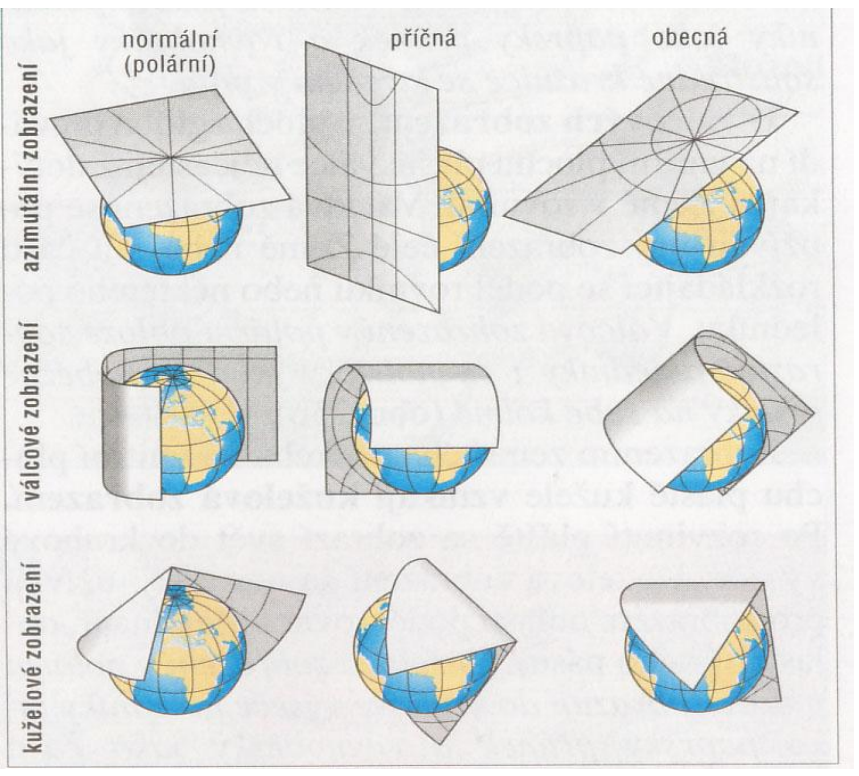
\includegraphics[width=0.7\textwidth]{uvod.png}
    \caption{Základní rozdělení kartografických zobrazení podle použité zobrazovací plochy (azimutální, válcové, kuželové - řádky) a její prostorové orientace vůči zemské ose (normální, příčná, obecná - sloupce). V této práci se zaměřujeme výhradně na optimalizaci zobrazení v obecné poloze (pravý sloupec). Zdroj: \parencite{gymmost}}
    \label{fig:typy_zobrazeni}
\end{figure}

\section{Zvolená zobrazení}
V této části budou představeny zvolené zobrazení, jejich zobrazovací rovnice a další teoretické výpočty a dosazení.

\subsection{Válcové konformní zobrazení}
Zobrazovací rovnice Mercatorova zobrazení v obecné poloze mají tvar:

$$x = c \cos d,$$
$$y = R \cdot \ln \tan\left(\frac{\check{s}}{2} + 45^\circ\right),$$

kde $c = R \cdot \cos(\check{s}_0)$. Volíme nezkreslenou rovnoběžku $\check{s}_0$ tak, aby byla hodnota zkreslení $\nu$ byla na severní $m^s_r$ a jižní $m^j_r$ rovnoběžce a na rovníku $m^r_r$až na znaménko stejná, tedy:

$$
m_r^s = m_r^j = 1 + \nu , \quad
m_r^r = 1 - \nu.
$$ 

Zeměpisnou šířku $\check{s}_0$ lze získat ze vztahu

$$\cos \check{s}_0 = \frac{2 \cos \check{s}_s}{1 + \cos \check{s}_s}.$$

Území je sevřeno do pásu svírající dvěma kartografickými rovnoběžkami tak, aby se jednalo o co neužší pás. Středem pásu je dále veden kartografický rovník. Na tomto rovníku jsou zvoleny dva libovolné body $P_1 = [u_1,u_1]$ a $P_2 = [u_2,u_2]$. Na okrajové rovnoběžce si zvolíme libovolný bod $P_3 = [u_3,u_3]$.

Pomocí kosínové věty pro sférický trojúhelník a dosazením našich bodů lze určit zeměpisné souřadnice karotgrafického pólu $K = [u_k,u_k]$:

$$\tan v_k = \frac{\tan u_1 \cos v_2 - \tan u_2 \cos v_1}{\tan u_2 \sin v_1 - \tan u_1 \sin v_2}$$
$$\tan u_k = -\frac{\cos(v_1 - v_k)}{\tan u_1} = -\frac{\cos(v_2 - v_k)}{\tan u_2}.
$$

Kartografickou šířku $\check{s}_s$ pro okrajovou rovnoběžku, na které leží bod $P_3$, určíme s použitím 1. kosínové věty:

$$\check{s}_s = \arcsin [\sin u_3 \sin u_k + \cos u_3 \cos u_k \cos(v_3 - v_k)].$$

Měřítko délek $m$ se v libovolném bodě s kartografickou šířkou $\check{s}$ určí ze vztahu 

$$m = m_p = m_r = \frac{\cos \check{s}_0}{\cos \check{s}} $$

a zkreslení délek jako 
$$\nu = m -1.$$

\subsection{Kuželové konformní zobrazení}
Zobrazovací rovnice Lambertova kuželového konformního zobrazení v obecné poloze mají tvar:
$$\rho = \rho_0 \frac{\tan^c\left(\frac{\check{s}_0}{2}+45^\circ\right)}{\tan^c\left(\frac{\check{s}}{2}+45^\circ\right)}$$
$$\epsilon = c \cdot d.$$

Zobrazení má dvě základní konstanty, $\rho_0$ a $c$. Tyto konstanty volíme z podmínky, aby hodnota zkreslení $\nu$ byla na severní okrajové rovnoběžce $m_r^s$, jižní okrajové rovnoběžce $m_r^j$ a ve středu území $m_r^0$ až na znaménko stejná, tedy:
$$
m_r^s = m_r^j = 1+\nu, \quad
m_r^0 = 1-\nu.
$$

Sečtením těchto vztahů získáme následující rovnici: 

$$c \rho_s \cos \check{s}_0 + c \rho_0 \cos \check{s}_s = 2R \cos \check{s}_0 \cos \check{s}_s.$$

Konstantu $\rho_0$ po dosazení určíme ze vzorce:
$$ \rho_0 = \frac{2R \cos \check{s}_0 \cos \check{s}_s \tan^c\left(\frac{\check{s}_s}{2} + 45^\circ\right)}{c\left[\cos \check{s}_0 \tan^c\left(\frac{\check{s}_0}{2} + 45^\circ\right) + \cos \check{s}_s \tan^c\left(\frac{\check{s}_s}{2} + 45^\circ\right)\right]}. $$

Konstantu $c$ a šířku nezkreslené rovnoběžky $\check{s}_0$ lze získat ze vztahů:
$$
c = \frac{\log \cos \check{s}_s - \log \cos \check{s}_j}{\log \tan\left(\frac{\check{s}_j}{2} + 45^\circ\right) - \log \tan\left(\frac{\check{s}_s}{2} + 45^\circ\right)}, \quad
\sin \check{s}_0 = c.
$$

Území je opět sevřeno do pásu pomocí dvou soustředních kružnic představující rovnoběžky. Střed kružnic $K = [u_k, v_k]$ je kartografický pól. Na každé z rovnoběžek vybereme libovolné body $P_1 = [u_1,u_1]$ (na severní r.) a $P_2 = [u_2,u_2]$ (na jižní r.). Jejich kartografické souřadnice pak vypočítáme z následujících vztahů:
$$
\check{s}_s = \arcsin [\sin u_1 \sin u_k + \cos u_1 \cos u_k \cos(v_1 - v_k)], $$
$$\check{s}_j = \arcsin [\sin u_2 \sin u_k + \cos u_2 \cos u_k \cos(v_2 - v_k)].$$

Výše vypočítané hodnoty dosadíme do obecného vzorce pro výpočet měřítka délek

$$m = m_p = m_r = \frac{c \rho_s}{R \cdot \cos u_s} = \frac{c \rho_j}{R \cdot \cos u_j} = 1 + \nu.$$

\subsection{Azimutální konformní zobrazení}
Zobrazovací rovnice stereografické projekce s jednou nezkreslenou rovnoběžkou v obecné poloze mají tvar:
$$\rho = c\cdot\tan\frac{\psi}{2} $$
$$\epsilon = d,$$
kde $\psi = 90^\circ - \check{s}$ představuje doplněk kartografické šířky do $90^\circ$. 

Konstanta zobrazení $c$ se určí ze vztahu 

$$c = 2R \cos^2 \frac{\psi_0}{2}.$$

Zobrazovací rovnice stereografické projekce s jednou nezkreslenou rovnoběžkou mají po přepsání pak tvar:

$$\rho = 2R \cos^2 \frac{\psi_0}{2} \tan \frac{\psi}{2}$$
$$\varepsilon = d$$


Pro území je vytvořena opasná kružnice s co nejmenším poloměrem. Střed kružnice $K = [u_k, v_k]$ je kartografický pól. Na rovnoběžce vybereme libovolný bod $P_1 = [u_1,u_1]$. Jeho kartografickou souřadnici pak vypočítáme z následujících vztahů:

$$ \check{s}_j = \arcsin [\sin u_1 \sin u_k + \cos u_1 \cos u_k \cos(v_1 - v_k)], $$

$$ \psi_j = 90^\circ - \check{s}_j. $$

V půlu nebudeme počítat s nulovým zkreslením, ale bude dosahovat hodnoty $\mu = 1 - \nu$, kde $\mu$ nazveme jako \textbf{multiplikační konstntu}. Nezkreslená rovnoběžka $\psi_0$ vyjde ze vztahu 

$$ m_r(\psi = 0) = \frac{\cos^2 \frac{\psi_0}{2}}{\cos^2 \frac{\psi}{2}} = \mu = 1 - \nu, $$

$$ \mu = \cos^2 \frac{\psi_0}{2} \Rightarrow \psi_0 = 2 \arccos \sqrt{\mu}. $$

Pokud budeme požadovat, aby hodnoty zkreslení $\gamma$ na rovnoběžce a v pólu byly až na znaménko stejné, pak platí 

$$ \mu = \frac{2 \cos^2 \frac{\psi_j}{2}}{1 + \cos^2 \frac{\psi_j}{2}}. $$

Měřítko délek $m_r,_j$ se pak pro rovnoběžku $\psi_j$ určí z

$$ m_{r,j} = \frac{\cos^2 \frac{\psi_0}{2}}{\cos^2 \frac{\psi_j}{2}}.$$

Výše zmíněné odvození a vzorce vycházely z návodu pro tuto úlohu \parencite{bayer}.

\section{Metodika určení parametrů zobrazení v GIS}

Pro konstrukci konformního zobrazení v obecné poloze je nezbytné nejprve definovat prostorovou orientaci kartografického rovníku (případně osy kužele či roviny) vůči referenční kouli. Protože matematický výpočet vyžaduje konkrétní souřadnice referenčních bodů, byla úvodní fáze optimalizace provedena v softwaru ArcGIS Pro nad generalizovanými vektorovými daty zkoumaných států (formát \texttt{.shp}).

\subsection{Parametry válcového zobrazení}

U válcového zobrazení je klíčové, aby nově definovaný kartografický rovník procházel podélnou osou území, čímž se minimalizuje vzdálenost okrajových bodů od tohoto rovníku, a tím i maximální délkové zkreslení na okrajích. Pro objektivní stanovení této osy byl v softwaru využit geoprocessingový nástroj \textit{Minimum Bounding Geometry}. Jako typ obalové geometrie byl zvolen opsaný obdélník definovaný šířkou (parametr \textit{Rectangle by Width}), který spolehlivě reflektuje dominantní směr extrémně protáhlých území, jakým je například Chile.

Získaný obdélník byl následně podélně rozpůlen, čímž vznikla centrální liniová osa reprezentující ideální průběh kartografického rovníku. Na této ose byly vizuálně odečteny geografické souřadnice dvou referenčních bodů ($P_1$, $P_2$), které jednoznačně definují její polohu v prostoru. Současně byly manuálně identifikovány a odečteny nejzazší okrajové body státní hranice ($P_3$, $P_4$). U kompaktních států bez dominantního směru (Švýcarsko) byl postup analogický, přičemž osa byla proložena středem největšího rozptylu hmoty území.

\begin{figure}[htbp]
    \centering
    \begin{minipage}{0.55\textwidth}
        \centering
        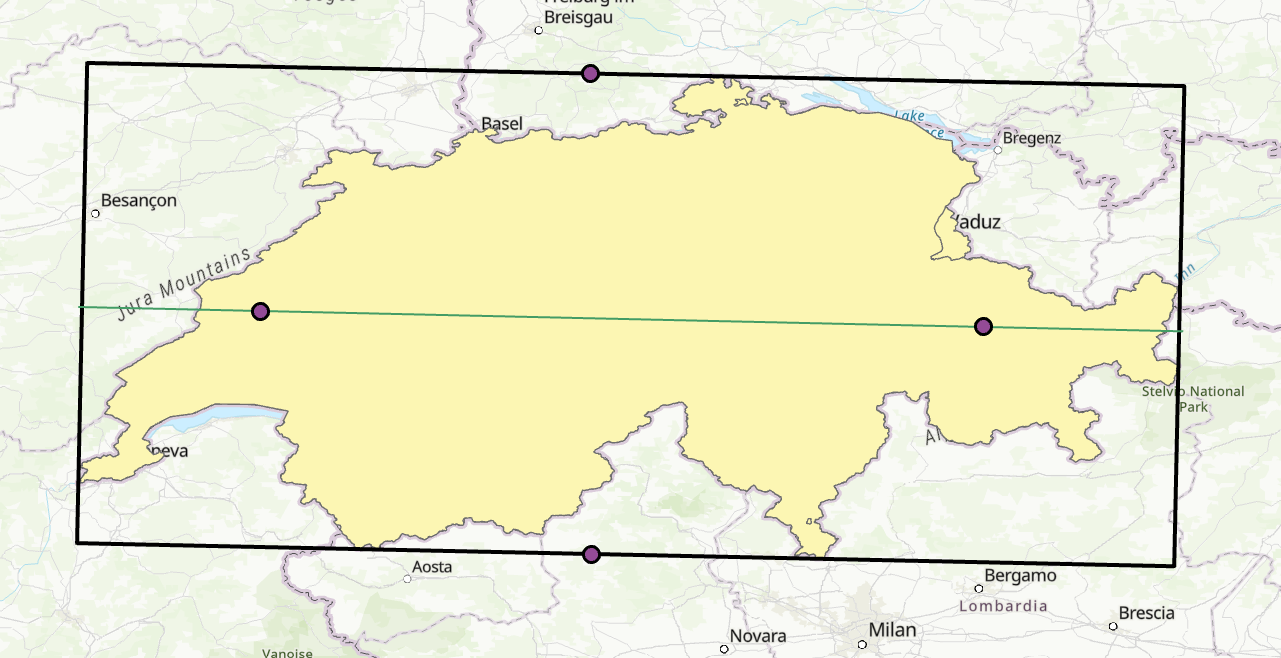
\includegraphics[width=\linewidth]{Swiss_new.png} 
        \caption{Určení osy a bodů pro Švýcarsko.}
    \end{minipage}\hfill
    \begin{minipage}{0.3\textwidth}
        \centering
        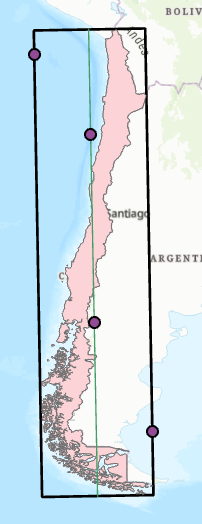
\includegraphics[width=\linewidth]{Chile.png}
        \caption{Určení osy a bodů pro Chile.}
    \end{minipage}
    \caption{Vizualizace odvození kartografického rovníku a okrajových bodů v prostředí ArcGIS Pro. Zelená linie reprezentuje osu území.}
    \label{fig:arcgis_metodika}
\end{figure}

\vspace{1.5em}
V Tabulce \ref{tab:vstupni_body_valec} jsou shrnuty geografické souřadnice (zeměpisná šířka $u$ a zeměpisná délka $v$) referenčních bodů odečtených pro konstrukci konformního válcového zobrazení v obecné poloze. Body $P_1$ a $P_2$ definují osu území (kartografický rovník), bod $P_3$ reprezentuje severní okraj a bod $P_4$ jižní okraj zkoumaného státu.


\begin{table}[htbp]
    \centering
    \newcolumntype{Y}{>{\centering\arraybackslash}X} 
    \begin{tabularx}{\textwidth}{|l|Y|Y|} 
        \hline
        \textbf{Bod} & \textbf{$u \ [^\circ]$} & \textbf{$v \ [^\circ]$} \\
        \hline
        \multicolumn{3}{|c|}{\textbf{Švýcarsko}} \\
        \hline
        $P_1$  & 46.839906 & 6.708829 \\
        $P_2$  & 46.774154 & 9.688181 \\
        $P_3$  & 47.797987 & 8.015539 \\
        $P_4$  & 45.819534 & 8.081614 \\
        \hline
        \multicolumn{3}{|c|}{\textbf{Chile}} \\
        \hline
        $P_1$  & -26.189752142 & -71.592771329 \\
        $P_2$  & -41.711194781 & -71.294470110 \\
        $P_3$  & -19.578328530 & -76.246879022 \\
        $P_4$  & -50.739861219 & -66.497675853 \\
        \hline
    \end{tabularx}
    \caption{Geografické souřadnice referenčních bodů z GIS pro válcové zobrazení.}
    \label{tab:vstupni_body_valec}
\end{table}

\subsection{Parametry kuželového zobrazení}
Práce pro výběr parametrů kuželového zobrazení probíhala v SW ArcGIS Pro. V této části bylo nutné vytvořit dvě \textbf{soustředné dotykové} kružnice kolem vybraných států. Důležité je zmínit, že byla snaha o dosáhnutí co nejmenšího rozdílu jejich poloměrů - tedy, že výsledný pás bude co nejužší.

Pro tvorbu těchto kružnic byla využita funkce \textit{Three Point Circle}, která vytvořila kružnici z tří vybraných bodů na hranici území (obrázek 5). Na těchto kružnicích byly dále zvoleny body $P_1$, který ležel na menší z kružnic, tudíž se jednalo o severnější bod a $P_2$, který ležel na vzdálenejší kružnici od kartografického pólu, tudíž se jedná o bod jižnější. Dále byl pomocí funkce \textit{Feature To Point} vytvořen střed kružnic, tedy \textbf{kartografický pól $P_k$}. Všechny výše zmíněné body a jejich souřadnice pro jednotlivé státy jsou vypsány v tabulce 2.

\begin{figure}[htbp]
    \centering
    \begin{subfigure}[b]{0.45\textwidth}
        \centering
        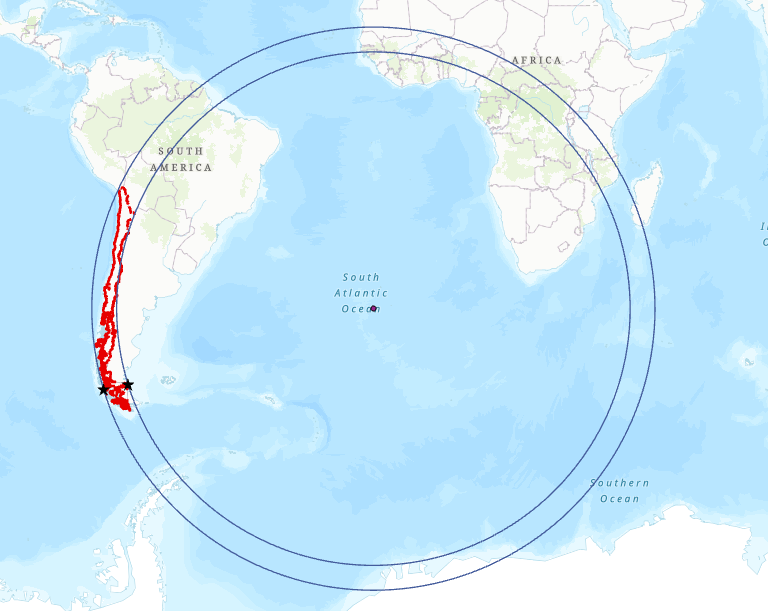
\includegraphics[width=\textwidth]{kuzel_kruz_chile.png}
        \caption{Chile}
        \label{fig:kuz_a}
    \end{subfigure}
    \hfill 
    \begin{subfigure}[b]{0.45\textwidth}
        \centering
        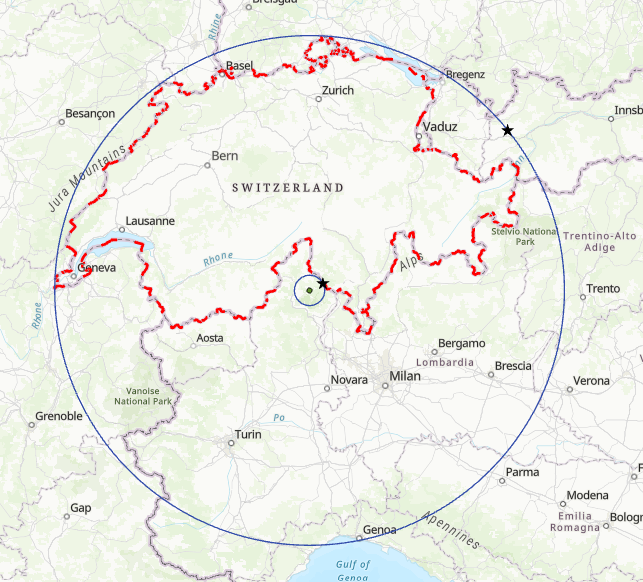
\includegraphics[width=\textwidth]{kuzel_kruz_svyc.png}
        \caption{Švýcarsko}
        \label{fig:kuz_b}
    \end{subfigure}
    \caption{Zvolené kružnice, středy a body pro kuželové zobrazení}
    \label{fig:all_kuz}
\end{figure}

\begin{table}[htbp]
    \centering
    \newcolumntype{Y}{>{\centering\arraybackslash}X} 
    \begin{tabularx}{\textwidth}{|l|Y|Y|} 
        \hline
        \textbf{Bod} & \textbf{$u \ [^\circ]$} & \textbf{$v \ [^\circ]$} \\
        \hline
        \multicolumn{3}{|c|}{\textbf{Švýcarsko}} \\
        \hline
        $P_k$  & 46.112849 & 8.448352 \\
        $P_1$  & 46.162395 & 8.578878 \\
        $P_2$  & 47.188548 & 10.383945 \\
        \hline
        \multicolumn{3}{|c|}{\textbf{Chile}} \\
        \hline        
        $P_k$  & -40.832077 & -13.909494 \\
        $P_1$  & -52.334372 & -68.417793 \\
        $P_2$  & -53.006039 & -73.851978 \\
        \hline
    \end{tabularx}
    \caption{Geografické souřadnice referenčních bodů z GIS pro kuželové zobrazení.}
    \label{tab:vstupni_body_kuzel}
\end{table}

\newpage

\subsection{Parametry azimutálního zobrazení}
Obdobně jako pro kuželové zobrazení, probíhala práce v SW ArcGIS Pro. V této části práce byly vytvořeny dotykové kružnice jednotlivých států. Důležité opět bylo, aby poloměr této kružnice byl co \textbf{nejmenší}.

Opět bylo využito funkce \textit{Three Point Circle}, která vytvořila zvolené dotykové kuržnice (obrázek 6). Na vytvořené kružnici byl tvolen bod $P_1$ a pomocí funkce \textit{Feature To Point} byl vytvřoen střed kružnice $P_k$. Souřadnice obou bodů jsou vypsány v tabulce 3 níže.

\begin{figure}[htbp]
    \centering
    \begin{subfigure}[b]{0.45\textwidth}
        \centering
        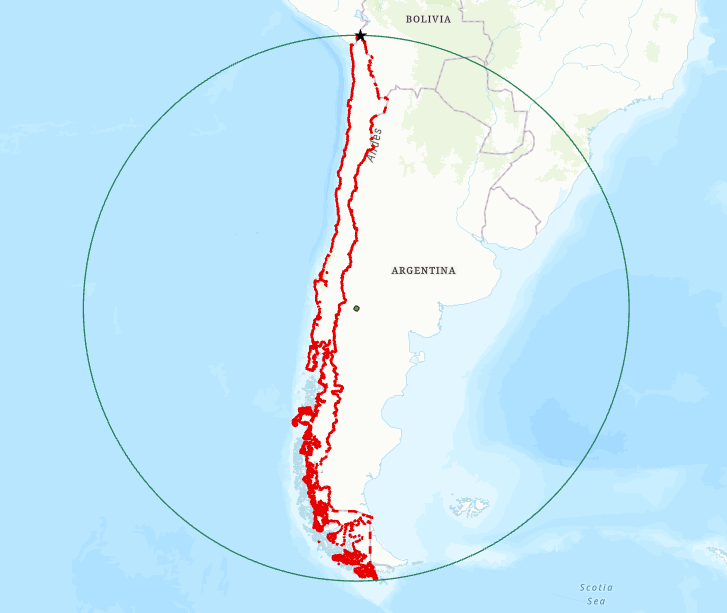
\includegraphics[width=\textwidth]{azim_kruz_chile.png}
        \caption{Chile}
        \label{fig:azi_a}
    \end{subfigure}
    \hfill 
    \begin{subfigure}[b]{0.45\textwidth}
        \centering
        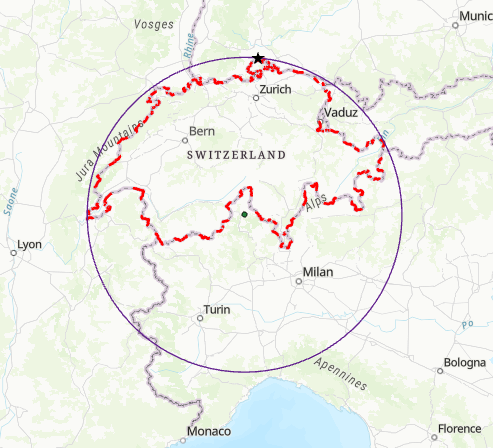
\includegraphics[width=\textwidth]{azim_kruz_svyc.png}
        \caption{Švýcarsko}
        \label{fig:azi_b}
    \end{subfigure}
    \caption{Zvolené kružnice, středy a body pro azimutální zobrazení}
    \label{fig:all_azi}
\end{figure}

\begin{table}[htbp]
    \centering
    \newcolumntype{Y}{>{\centering\arraybackslash}X} 
    \begin{tabularx}{\textwidth}{|l|Y|Y|} 
        \hline
        \textbf{Bod} & \textbf{$u \ [^\circ]$} & \textbf{$v \ [^\circ]$} \\
        \hline
        \multicolumn{3}{|c|}{\textbf{Švýcarsko}} \\
        \hline
        $P_k$  & 46.172893 & 8.3603224 \\
        $P_1$  & 47.805634 & 8.566455 \\
        \hline
        \multicolumn{3}{|c|}{\textbf{Chile}} \\
        \hline        
        $P_k$  & -39.149663 & -69.870458 \\
        $P_1$  & -17.498348 & -69.468452 \\
        \hline
    \end{tabularx}
    \caption{Geografické souřadnice referenčních bodů z GIS pro azimutální zobrazení.}
    \label{tab:vstupni_body_azim}
\end{table}

\newpage

\section{Výpočetní část}

V této kapitole jsou popsány matematické postupy a algoritmy využité pro transformaci souřadnic a výpočet délkového zkreslení. Veškeré iterativní a analytické procesy byly programovány v jazyce Python bez použití pokročilých výpočetních knihoven (např. NumPy).

\subsection{Válcové konformní zobrazení (Mercator)}



\subsubsection{Exaktní optimalizace dotykové rovnoběžky (Iterativní algoritmus)}

Klasický přístup výpočtu dotykové rovnoběžky $\check{s}_0$ spoléhá na manuální odečet okrajového bodu $P_3$ v prostředí GIS. Tento postup je však silně náchylný k chybě lidského faktoru, což může vést k neoptimální nastavení měřítka. Pro eliminaci tohoto jevu a dosažení absolutní matematické přesnosti byl nad rámec zadán, jako bonus, implementován iterativní vyhledávací algoritmus.

Tento algoritmus využívá knihovnu \texttt{shapefile} pro načtení všech lomových bodů polygonu reprezentujícího státní hranici. Geografické souřadnice každého bodu ($u_i, v_i$) jsou pomocí sférické kosinové věty transformovány na kartografickou šířku $\check{s}_i$ vůči předem vypočtenému analytickému pólu $K$. Algoritmus následně prochází celou množinu bodů a vyhledá bod s absolutně největší kartografickou šířkou:
$$ \check{s}_{s(exact)} = \max(| \check{s}_i |) $$

Tato exaktně zjištěná hodnota je následně dosazena do rovnice pro výpočet optimální dotykové rovnoběžky $\check{s}_{0(exact)}$. 

\paragraph{Návrh iterativního algoritmu}
Logika vyhledávání extrémní kartografické šířky ze zdrojového souboru \texttt{.shp} je postavena na principu průchodu všech vrcholů polygonu. Pro každý bod je vypočtena jeho vzdálenost od kartografického rovníku a porovnána s dosavadním maximem. Zjednodušený pseudokód algoritmu vypadá následovně:
\vspace{1.5em}

\hline
\begin{verbatim}
Algoritmus: Najdi_Extremni_Sirku(shapefile, u_k, v_k)
1. Inicializuj max_s = 0.0
2. Pro každý polygon VE shapefile:
3.     Peo každý bod (lon, lat) V polygonu:
4.         Převeď lat, lon na radiány (u, v)
5.         Spočítej kartografickou šířku 's' vůči pólu (u_k, v_k)
6.         Pokud absolutní_hodnota(s) > max_s:
7.             max_s = absolutní_hodnota(s)
8. Vrať max_s
\end{verbatim}

\vspace{1.5em}

Tento jednoduchý, avšak výpočetně robustní cyklus zaručuje detekci absolutního maxima bez ohledu na orientaci a složitost polygonu státní hranice.

\subsection{Celkové zhodnocení válcového zobrazení}

V této sekci jsou porovnány výsledné hodnoty délkového zkreslení a klíčových parametrů zobrazení (kartografický pól $K$ a nezkreslená rovnoběžka $\check{s}_0$) pro státy Chile a Švýcarsko. Výsledky rovněž demonstrují rozdíl mezi manuálním určením parametrů v prostředí ArcGIS a exaktním iterativním algoritmem nad soubory \texttt{.shp}.

\subsubsection{Poloha kartografického pólu}

V Tabulce \ref{tab:pol_k_porovnani} je zobrazeno srovnání výpočtu kartografického pólu $K$ pomocí tradiční sférické trigonometrie a alternativní 3D analytické geometrie. U obou testovaných států vykazují obě metody naprostou shodu s přesností přesahující 14 desetinných míst. Tento výsledek plně verifikuje geometrickou stabilitu implementovaných algoritmů.

\begin{table}[htbp]
    \centering
    \renewcommand{\arraystretch}{1.2}
    \begin{tabular}{|l|c|c|c|}
        \hline
        \textbf{Stát} & \textbf{Výpočetní metoda} & \textbf{$u_K \ [^\circ]$} & \textbf{$v_K \ [^\circ]$} \\
        \hline
        \multirow{2}{*}{\textbf{Chile}} & Sférická trigonometrie & 0.746652 & 18.039973 \\
        & 3D analytická geometrie & 0.746652 & 18.039973 \\
        \hline
        \multirow{2}{*}{\textbf{Švýcarsko}} & Sférická trigonometrie & 43.155365 & -174.333260 \\
        & 3D analytická geometrie & 43.155365 & -174.333260 \\
        \hline
    \end{tabular}
    \caption{Porovnání metod výpočtu kartografického pólu $K$.}
    \label{tab:pol_k_porovnani}
\end{table}

\subsubsection{Analýza délkového zkreslení}
Klíčovým parametrem pro posouzení kvality zobrazení je hodnota délkového zkreslení na kontrolních bodech. V Tabulkách \ref{tab:zkresleni_chile} a \ref{tab:zkresleni_svycarsko} jsou uvedeny srovnávací hodnoty pro manuálně definovaný okraj a okraj zjištěný iterativním exaktním průchodem vektorových dat.


\clearpage
\newpage


\begin{table}[htbp]
    \centering
    \renewcommand{\arraystretch}{1.2}
    \begin{tabular}{|l|c|c|}
        \hline
        \textbf{Bod} & \textbf{Manuální odečet z ArcGIS} & \textbf{Exaktní iterace (Shapefile)} \\
        \hline
        Dotyková rovnoběžka $\check{s}_0$ & $3,034618^\circ$ & $3,028815^\circ$ \\
        \hline
        Zkreslení $P_1$  [m/km] & -1,402268 & -1,396912 \\
        Zkreslení $P_2$  [m/km] & -1,402268 & -1,396912 \\
        Zkreslení $P_3$  [m/km] & 1,402268 & 1,407640 \\
        Zkreslení $P_4$  [m/km] & -0,144327 & -0,138963 \\
        \hline
    \end{tabular}
    \caption{Porovnání parametrů a délkového zkreslení pro \textbf{Chile}.}
    \label{tab:zkresleni_chile}
\end{table}

\begin{table}[htbp]
    \centering
    \renewcommand{\arraystretch}{1.2}
    \begin{tabular}{|l|c|c|}
        \hline
        \textbf{Bod} & \textbf{Manuální odečet z ArcGIS} & \textbf{Exaktní iterace (Shapefile)} \\
        \hline
        Dotyková rovnoběžka $\check{s}_0$ & $0,690825^\circ$ & $0,706992^\circ$ \\
        \hline
        Zkreslení $P_1$  [m/km] & -0,072687 & -0,076129 \\
        Zkreslení $P_2$  [m/km] & -0,072687 & -0,076129 \\
        Zkreslení $P_3$  [m/km] & 0,072687 & 0,069244 \\
        Zkreslení $P_4$  [m/km] & 0,079395 & 0,075953 \\
        \hline
    \end{tabular}
    \caption{Porovnání parametrů a délkového zkreslení pro \textbf{Švýcarsko}.}
    \label{tab:zkresleni_svycarsko}
\end{table}

\subsubsection{Vyhodnocení} 

Z celkového hlediska je nutné hodnotit konformní válcové zobrazení v obecné poloze vždy v kontextu tvaru a rozlohy daného státu. 

V případě extrémně protáhlého území Chile dosahuje maximální délkové zkreslení hodnoty přibližně $1,4$~m/km. V absolutních měřítkách se již jedná o nezanedbatelnou deformaci (na každý reálný kilometr narůstá chyba na mapě o 1,4 metru). Nicméně vzhledem k extrémní délce tohoto státu, která přesahuje 4300 km, jde o matematicky nevyhnutelný a v celostátním měřítku akceptovatelný kompromis, pokud požadujeme zobrazení celého území v jediném souvislém souřadnicovém pásu. 

Naopak pro sféricky kompaktní území Švýcarska se toto zobrazení jeví jako ideální. Zkreslení se zde na okrajích pohybuje pod hranicí $0,08$~m/km (což představuje deformaci pouhých 8 centimetrů na jeden kilometr).

\subsubsection{Popis vytvořených skriptů a funkcí}

Pro správný chod a výpočet parametrů Mercatorova zobrazení byly vytvořeny výpočetní skripty v jazyce Python. Vzhledem k matematické povaze úlohy nebylo nutné využívat objektově orientovanou architekturu, kód je však pro maximální přehlednost rozdělen do samostatných pomocných funkcí a hlavního výpočetního bloku. Níže je popsána struktura hlavního skriptu \texttt{merc\_chile.py}.

\subsubsection{Pomocné analytické funkce}

\begin{itemize}
    \item \textbf{geo\_to\_xyz}: Zajišťuje převod geografických úhlů (zeměpisné šířky a délky v radiánech) na prostorový 3D vektor na jednotkové kouli.
    
    \item \textbf{my\_cross\_product}: Realizuje výpočet vektorového součinu dvou 3D vektorů pro nalezení kolmé normály.
    
    \item \textbf{uvToSd}: Transformuje standardní geografické souřadnice zadaného bodu do kartografických souřadnic šikmého aspektu vůči nově vypočtenému pólu $K$. Metoda vrací hledanou kartografickou šířku $s$.
    
    \item \textbf{find\_extreme\_s}: Samostatná iterativní metoda (importovaná z pomocného modulu). Načítá definovaný soubor \texttt{.shp}, cyklicky prochází veškeré lomové body polygonu státní hranice a vrací absolutně největší zjištěnou kartografickou šířku.
\end{itemize}

\subsubsection{Hlavní výpočetní blok skriptu}

\begin{itemize}
    \item \textbf{Definice vstupů}: Inicializuje úhlové hodnoty referenčních bodů $P_1$ až $P_4$ (odečtených z prostředí GIS) a převádí je ze stupňů na radiány.
    
    \item \textbf{Výpočet pólu K}: Paralelně provádí stanovení polohy kartografického pólu nejprve pomocí tradiční sférické trigonometrie a následně i pomocí 3D analytické geometrie (kombinací funkcí \texttt{geo\_to\_xyz} a \texttt{my\_cross\_product}) pro vzájemnou verifikaci.
    
    \item \textbf{Výpočet dotykové rovnoběžky}: Aplikuje kosinovou větu pro zjištění šířky standardní rovnoběžky $s_0$ na základě manuálně odečteného bodu. Následně spouští funkci \texttt{find\_extreme\_s} pro výpočet exaktní rovnoběžky $s_{0(exact)}$.
    
    \item \textbf{Analýza zkreslení}: Počítá finální délková měřítka $m$ a zkreslení $\nu$ pro manuální i exaktní optimalizační přístup a formátuje výsledky pro zápis do tabulek.
\end{itemize}

\vspace{0.5cm}
\noindent \textit{Poznámka:} Logika, použité funkce a struktura výše popsaného skriptu jsou naprosto totožné i pro druhý zkoumaný stát (Švýcarsko). Skript \texttt{merc\_switzerland.py} se odlišuje výhradně ve vstupních parametrech úvodní definice bodů a v cestě k příslušnému zdrojovému souboru \texttt{.shp}.

\subsection{Algoritmus pro kuželové konformní zobrazení (Lambert)}

Skript pro kuželové zobrazení (\texttt{lcc.py}) analyticky řeší hledání konstanty kužele a optimálních poloměrů.
\begin{itemize}
    \item \textbf{Zpracování vstupů:} Do skriptu vstupují předem zjištěné souřadnice pólu $K$ a dvou bodů ležících na severní a jižní ohraničující kružnici, které jsou vzápětí transformovány do obecné polohy ($s_1$, $s_2$).
    \item \textbf{Výpočet konstant a poloměrů:} Hlavní konstanta zobrazení $c$ je vypočtena podle teoretických vzorců. Z této konstanty je funkcí \texttt{asin} zpětně získána šířka nezkreslené rovnoběžky $s_0$ a odvozeny příslušné poloměry $\rho_0$, $\rho_1$ a $\rho_2$.
    \item \textbf{Vyhodnocení zkreslení:} Pomocí funkce \texttt{round(..., 6)} jsou výsledné hodnoty délkového zkreslení na obou okrajích a ve středu zaokrouhleny na 6 desetinných míst.
\end{itemize}

\subsubsection{Vyhodnocení zobrazení}

Hodnoty zkreslení $\nu$ z tabulky 7 ukazují skvělé výsledky. Pro lepší představivost jsou původní výsledky ($\nu$) vynásobeny 1000 a tudíž převedeny na metry na jeden kilometr ($m/km$).

Pro extrémně protáhlé \textbf{Chile} představuje kuželové zobrazení naprosto dokonalé řešení. Celé území se do tohoto úzkého pruhu bez problému vejde, díky čemuž zkreslení dosahuje pohých $\nu = 0,195056$. V praxi to znamená zanedbatelnou deformaci pouhých 20 centimetrů na kilometr ($0,2~m/km$).

I v případě \textbf{Švýcarska} dosáhlo kuželové zobrazení výborných výsledků, dokonce nejlepších z celého měření – pouhých $\nu = 0,057392$. To odpovídá chybě necelých 6 centimetrů na kilometr ($0,06~m/km$). Není to však proto, že by byl pás pro tvar Švýcarska výhodnější než kružnice, ale primárně proto, že je Švýcarsko plošně velmi malé oproti Chile. Svírající pás mohl být nastaven jako extrémně úzký, což logicky snížilo zkreslení na velmi malou hodnotu.

\begin{table}[htbp]
    \centering
    \begin{tabular}{|l|c|c|}
        \hline
        \textbf{Rovnoběžka} & \textbf{Chile} & \textbf{Švýcarsko} \\
        \hline
        severní & 0,195056 & 0,057392 \\
        jižní & 0,195056 & 0,057392 \\
        středová & -0,195056 & -0,057392 \\
        \hline
    \end{tabular}
    \caption{Zkreslení kuželového zobrazení}
    \label{tab:kuzel_zkresleni}
\end{table}


\subsection{Algoritmus pro azimutální konformní zobrazení}
Skript pro stereografickou projekci (\texttt{stereo\_proj.py}) optimalizuje zobrazení zavedením multiplikační konstanty.
\begin{itemize}
    \item \textbf{Vstupy:} Vstupem je střed opsané kružnice $K$ a jeden bod definující okrajovou rovnoběžku. Po provedení prostorové transformace do obecné polohy se vypočítá doplňkový úhel $\psi$ ( $\pi/2 - s_1$).
    \item \textbf{Multiplikační konstanta:} Aby platila podmínka rovnosti hodnot zkreslení v pólu a na okraji, vypočte algoritmus multiplikační konstantu $\mu$. Následně je odvozena teoretická poloha nezkreslené kružnice $\psi_0$.
    \item \textbf{Dopočet zkreslení:} Měřítko na okraji i ve středu území je dopočteno podle teoretických vzorců a pak je dopočteno vlastní zkreslení $\nu$. Výsledek je pak zaokrouhlen na 6 desetinných míst.
\end{itemize}

\subsubsection{Vyhodnocení zobrazení}

Výsledné hodnoty zkreslení ($\nu$) v tabulce 8 ukazují, jak tvar státu ovlivňuje použitelnost tohoto zobrazení. Pro lepší představivost lze hodnotu zkreslení opět převést na metry na jeden kilometr ($m/km$).

Azimutální zobrazení je pro \textbf{Chile} naprosto nevhodné. Vzhledem k extrémní délce státu musí mít opsaná kružnice obrovský poloměr. Okraje území jsou příliš daleko od kartografického pólu (středu kružnice), což vede k obrovskému zkreslení $\nu = 0,017960$. V reálu to znamená, že mapa je na okrajích deformována chybou téměř 18 metrů na každý kilometr ($17,96~m/km$).

Pro \textbf{Švýcarsko} je azimutální zobrazení naopak naprosto ideální. Území má kompaktní tvar, který se přirozeně blíží kruhu, a do opsané kružnice zapadne velmi těsně. Vzdálenost od středu k okrajům je malá, díky čemuž je zkreslení minimální – pouze $\nu = 0,102264$. To v praxi představuje malé zkreslení pouhých 10 centimetrů na kilometr ($0,1~m/km$).

\begin{table}[htbp]
    \centering
    \begin{tabular}{|l|c|c|}
        \hline
        \textbf{Rovnoběžka} & \textbf{Chile} & \textbf{Švýcarsko} \\
        \hline
        dotyková & 17,959812 & 0,102264 \\
        pól & -17,959812 & -0,102264 \\
        \hline
    \end{tabular}
    \caption{Azimutální zobrazení -- délkové zkreslení $\nu$}
    \label{tab:azimut_zkresleni}
\end{table}

\section{Závěr}
Úkolem této úlohy bylo detailní porovnání délkového zkreslení tří základních konformních kartografických zobrazení (válcového, kuželového a azimutálního) v obecné poloze. Pro objektivní zhodnocení byly záměrně vybrány dva tvarově odlišné státy: Chile (s dominantním směrem) a Švýcarsko (kompaktní území).

Získané výsledky jednoznačně potvrdily závislost mezi tvarem území a vhodností zvoleného zobrazení. Pro extrémně protáhlé území Chile se jako nejvhodnější ukázalo kuželové zobrazení, které dosáhlo zkreslení pouhých $\nu = 0,195056$ (tedy $0,2~m/km$). Válcové zobrazení orientované podél podélné osy území generovalo zkreslení okolo $1,4~m/km$, což je pro takto dlouhý stát stále skvělý výsledek. Naopak azimutální zobrazení u Chile zcela selhalo z důvodu svého tvaru. Výsledkem bylo extrémní zkreslení $\nu = 17,959812$ (téměř $18~m/km$).

U kompaktního území Švýcarska dosahovala všechna tři zobrazení vynikajících výsledků s deformacemi v řádech pouhých centimetrů na kilometr. Přestože pro Švýcarsko matematicky vycházelo nejlépe také kuželové zobrazení ($\nu = 0,057392$), z logického hlediska je pro tento kruhový tvar nejpřirozenější volbou zobrazení azimutální ($\nu = 0,102264$). 

Z těchto výsledků lze vyvodit obecné pravidlo: pro státy s jedním výrazným dominantním směrem je vhodné volit zobrazení kuželová či válcová orientovaná podél osy území, zatímco pro kompaktní státy bez dominantního směru je optimální volbou zobrazení azimutální.

Jako bonus byl do skriptů přidán algoritmus, který automaticky vyhledává potřebné body hranice přímo ze souboru \textit{.shp}. Tím se eliminovaly chyby a nepřesnosti, které vznikají při ručním odečítání souřadnic. Nad rámec zadání byl také kartografický pól vypočítán pomocí analytické geometrie, což posloužilo jako spolehlivá kontrola pro předchozí výpočty.

\printbibliography[title=Zdroje]

\end{document}





